\documentclass[11pt,titlepage]{article}

\usepackage{geometry}
\geometry{
    a4paper,
    total={210mm,297mm},
    left=20mm,
    right=20mm,
    top=20mm,
    bottom=50mm,
}

% Polski
\usepackage[]{polski} 
\usepackage[polish]{babel}

% Pierwszy akapit - wcięty
\usepackage[]{indentfirst}

% Matematyka
\usepackage[]{amsfonts}
\usepackage[]{amsmath}

% Formatowanie
\usepackage{ragged2e}

% Tytuły sekcji na środku
\usepackage{titlesec}
% \titleformat{\section}[block]{\Large\bfseries\filcenter}{}{1em}{}

% <=
\usepackage{amssymb}

% eps
\usepackage{graphicx}

% Tabele
\usepackage{array}
\usepackage{makecell}

%""
\usepackage[style=czech]{csquotes}

% ref
\usepackage[backend=biber,style=numeric,sorting=none]{biblatex}
\addbibresource{bib.bib}

% POC
\usepackage{epstopdf}
\usepackage{standalone}
\usepackage{tikz}
\usepackage{tabularx}
\usepackage{subfig}

% Wykres
\usepackage{textcomp}
\usepackage{pgfplots}
\pgfplotsset{width=10cm,compat=1.9}

% Import
\usepackage{import}

\renewcommand*{\thesubsubsection}{}

\usepackage{hyperref}
\hypersetup{
    colorlinks,
    citecolor=black,
    filecolor=black,
    linkcolor=black,
    urlcolor=black
}

\usepackage{listings}
\usepackage{xcolor}

\lstset{language=C++}
\lstdefinestyle{MyC++Style} {
    language=C++,
    basicstyle=\footnotesize\ttfamily,
    breakatwhitespace=false,
    breaklines=true,
    commentstyle=\color{gray},
    extendedchars=true,
    frame=single,
    keepspaces=true,
    keywordstyle=\color{orange},
    numbers=left,
    numbersep=5pt,
    numberstyle=\footnotesize\color{gray},
    rulecolor=\color{black},
    rulesepcolor=\color{blue},
    showspaces=false,
    showstringspaces=false,
    showtabs=false,
    stringstyle=\color{orange},
    tabsize=2,
    emphstyle=\bfseries\color{blue}%  style for emph={} 
}

% svg
\usepackage{svg}

\usepackage{fancyhdr}
\pagestyle{fancy}
\headheight=98pt
\fancyhead[L]{\includegraphics[scale=0.3]{img/politechnika_sl_logo_bw_poziom_pl.eps}}
\fancyhead[C]{Podstawy Robotyki \\ Ramię robota\vspace{0.4cm}}
\fancyhead[R]{Siedliski, Tchórzewski, \\ Davis, Mendzik, Kula \vspace{0.4cm}}
\fancyfoot[C]{\thepage}

% Pozioma strona
\usepackage{pdflscape}

% Stackowanie
\usepackage{stackengine}

\renewcommand{\headrulewidth}{1pt}
\renewcommand{\footrulewidth}{1pt}

\title{
\includegraphics[scale=0.75]{img/politechnika_sl_logo_bw_poziom_pl.eps}\\
\textbf{Wydział Automatyki, Elektroniki\\
i Informatyki}\\
\vspace*{1cm}
Podstawy Robotyki
}
\author{Mateusz Siedliski\\
Radosław Tchórzewski\\
Paweł Mendzik\\
Jakub Kula\\
Oliver Davis}
\date{Gliwice 2023}

\begin{document}

\maketitle

\tableofcontents

\newpage

\listoffigures

\listoftables

\printbibliography

\newpage

\section{Wstęp}

Główną inspiracją projektu był film zamieszczony na platformie YouTube z kanału \enquote{How To Mechatronics} pod tytułem \enquote{DIY Arduino Robot Arm with Smartphone Control} \cite*{HTM_YT}.

Nasz projekt korzysta z tych samych technologii, aczkolwiek wszystkie elementy (model 3D, oprogramowanie mikrokontrolera, kod aplikacji, schemat połączeń itd.) zostały przygotowane przez nas.

W ramach projektu stworzono dydaktyczny model 5 osiowego manipulatora z chwytakiem, zrealizowanego w technologii druku 3D, sterowany aplikacją na urządzenia mobilne z systemem Android.

\subsection{Cel i zakres projektu}

\subsubsection{Cel projektu}

Celem projektu była realizacja fizycznego modelu manipulatora przeznaczonego do celów dydaktycznych. Może być on pomocny dla studentów w celu wizualizacji koncepcji teoretycznych w prawdziwym świecie, a nie tylko w książkach, czy na ekranie komputera.

\section{Urządzenie wraz z aplikacją}

\subsection{Wykonanie}

\subsubsection{Wybór elementów}

Prace rozpoczęto od doboru elementów elektronicznych i mechanicznych oraz wyboru procesu technologicznego wykonania manipulatora:

\begin{itemize}
    \item M5Stack Core2 — ESP32-D0WD-V3
    \item PCA9685PW — 16 kanałowy 12-Bit sterownik I$^2$C PWM serwo
    \item Micro Servo 9g SG90
    \item Servo Mg996r
    \item Obudowa ramienia (druk 3D)
    \item Przewody
    \item Wkręty M3
    \item Śruby M3
    \item Nakrętki M3
    \item Drewniana podstawa
\end{itemize}

\medskip

Jako proces technologiczny wykorzystany do stworzenia korpusu urządzenia wybrano druk 3D ze względu na niski koszt i powszechną dostępność. Technologia ta również umożliwia optymalizację procesu twórczego poprzez wielokrotne iteracje.

\newpage

\subsubsection{Model 3D}

Następnym krokiem było zaprojektowanie modelu 3D manipulatora przy użyciu programu \\ \href{https://www.autodesk.pl/products/fusion-360}{\underline{Autodesk Fusion 360}\footnote{Zintegrowane oprogramowanie CAD, CAM, CAE i PCB}}.

Program Autodesk Fusion 360 to bardzo przystępna alternatywa dla środowiska Autodesk Inventor. Przy braku poprzedniego doświadczenia autorzy byli w stanie całkowicie od zera zaprojektować i zrealizować w pełni działający model manipulatora. Proces tworzenia korpusu pokazano na Rysunkach \ref{Modelowanie3Dleft} i \ref{Modelowanie3Dtop}\footnote{Wizualizacje stworzono w programie \href{https://www.blender.org}{\underline{Blender}}}, a gotowy model przedstawiono na Rysunku \ref{AutodeskViewer}.

\begin{figure}[h!]
    \begin{center}
        \includegraphics[width=0.7\textwidth]{img/leftW.png}
    \end{center}
    \begin{center}
        \includegraphics[width=0.7\textwidth]{img/leftC.png}
    \end{center}
    \caption{Proces tworzenia modelu 3D — Widok z boku}
    \label{Modelowanie3Dleft}
\end{figure}

\begin{figure}[p]
    \begin{center}
        \includegraphics[width=0.4\textwidth]{img/topW.png}
        \includegraphics[width=0.4\textwidth]{img/topC.png}
    \end{center}
    \caption{Proces tworzenia modelu 3D — Widok z góry}
    \label{Modelowanie3Dtop}
\end{figure}

\begin{figure}[p]
    \vspace{1cm}
    \begin{center}
        \includegraphics[width=0.9\textwidth]{img/Robak v25.f3d.png}
    \end{center}
    \caption[Gotowy model w programie
        \href{https://viewer.autodesk.com/}
        {\underline{Autodesk Viewer}}]
    {Gotowy model w programie
        \href{https://viewer.autodesk.com/}
        {\underline{Autodesk Viewer}} \\ Narzędzie online do wyświetlania plików 2D i 3D}
    \label{AutodeskViewer}
\end{figure}

\newpage

\subsubsection{Konstrukcja mechaniczna}

Model złożono przy użyciu śrub, wkrętów i nakrętek M3, co przedstawiono na Rysunkach \ref{mechC} i \ref{mechB}.

\begin{figure}[h!]
    \begin{center}
        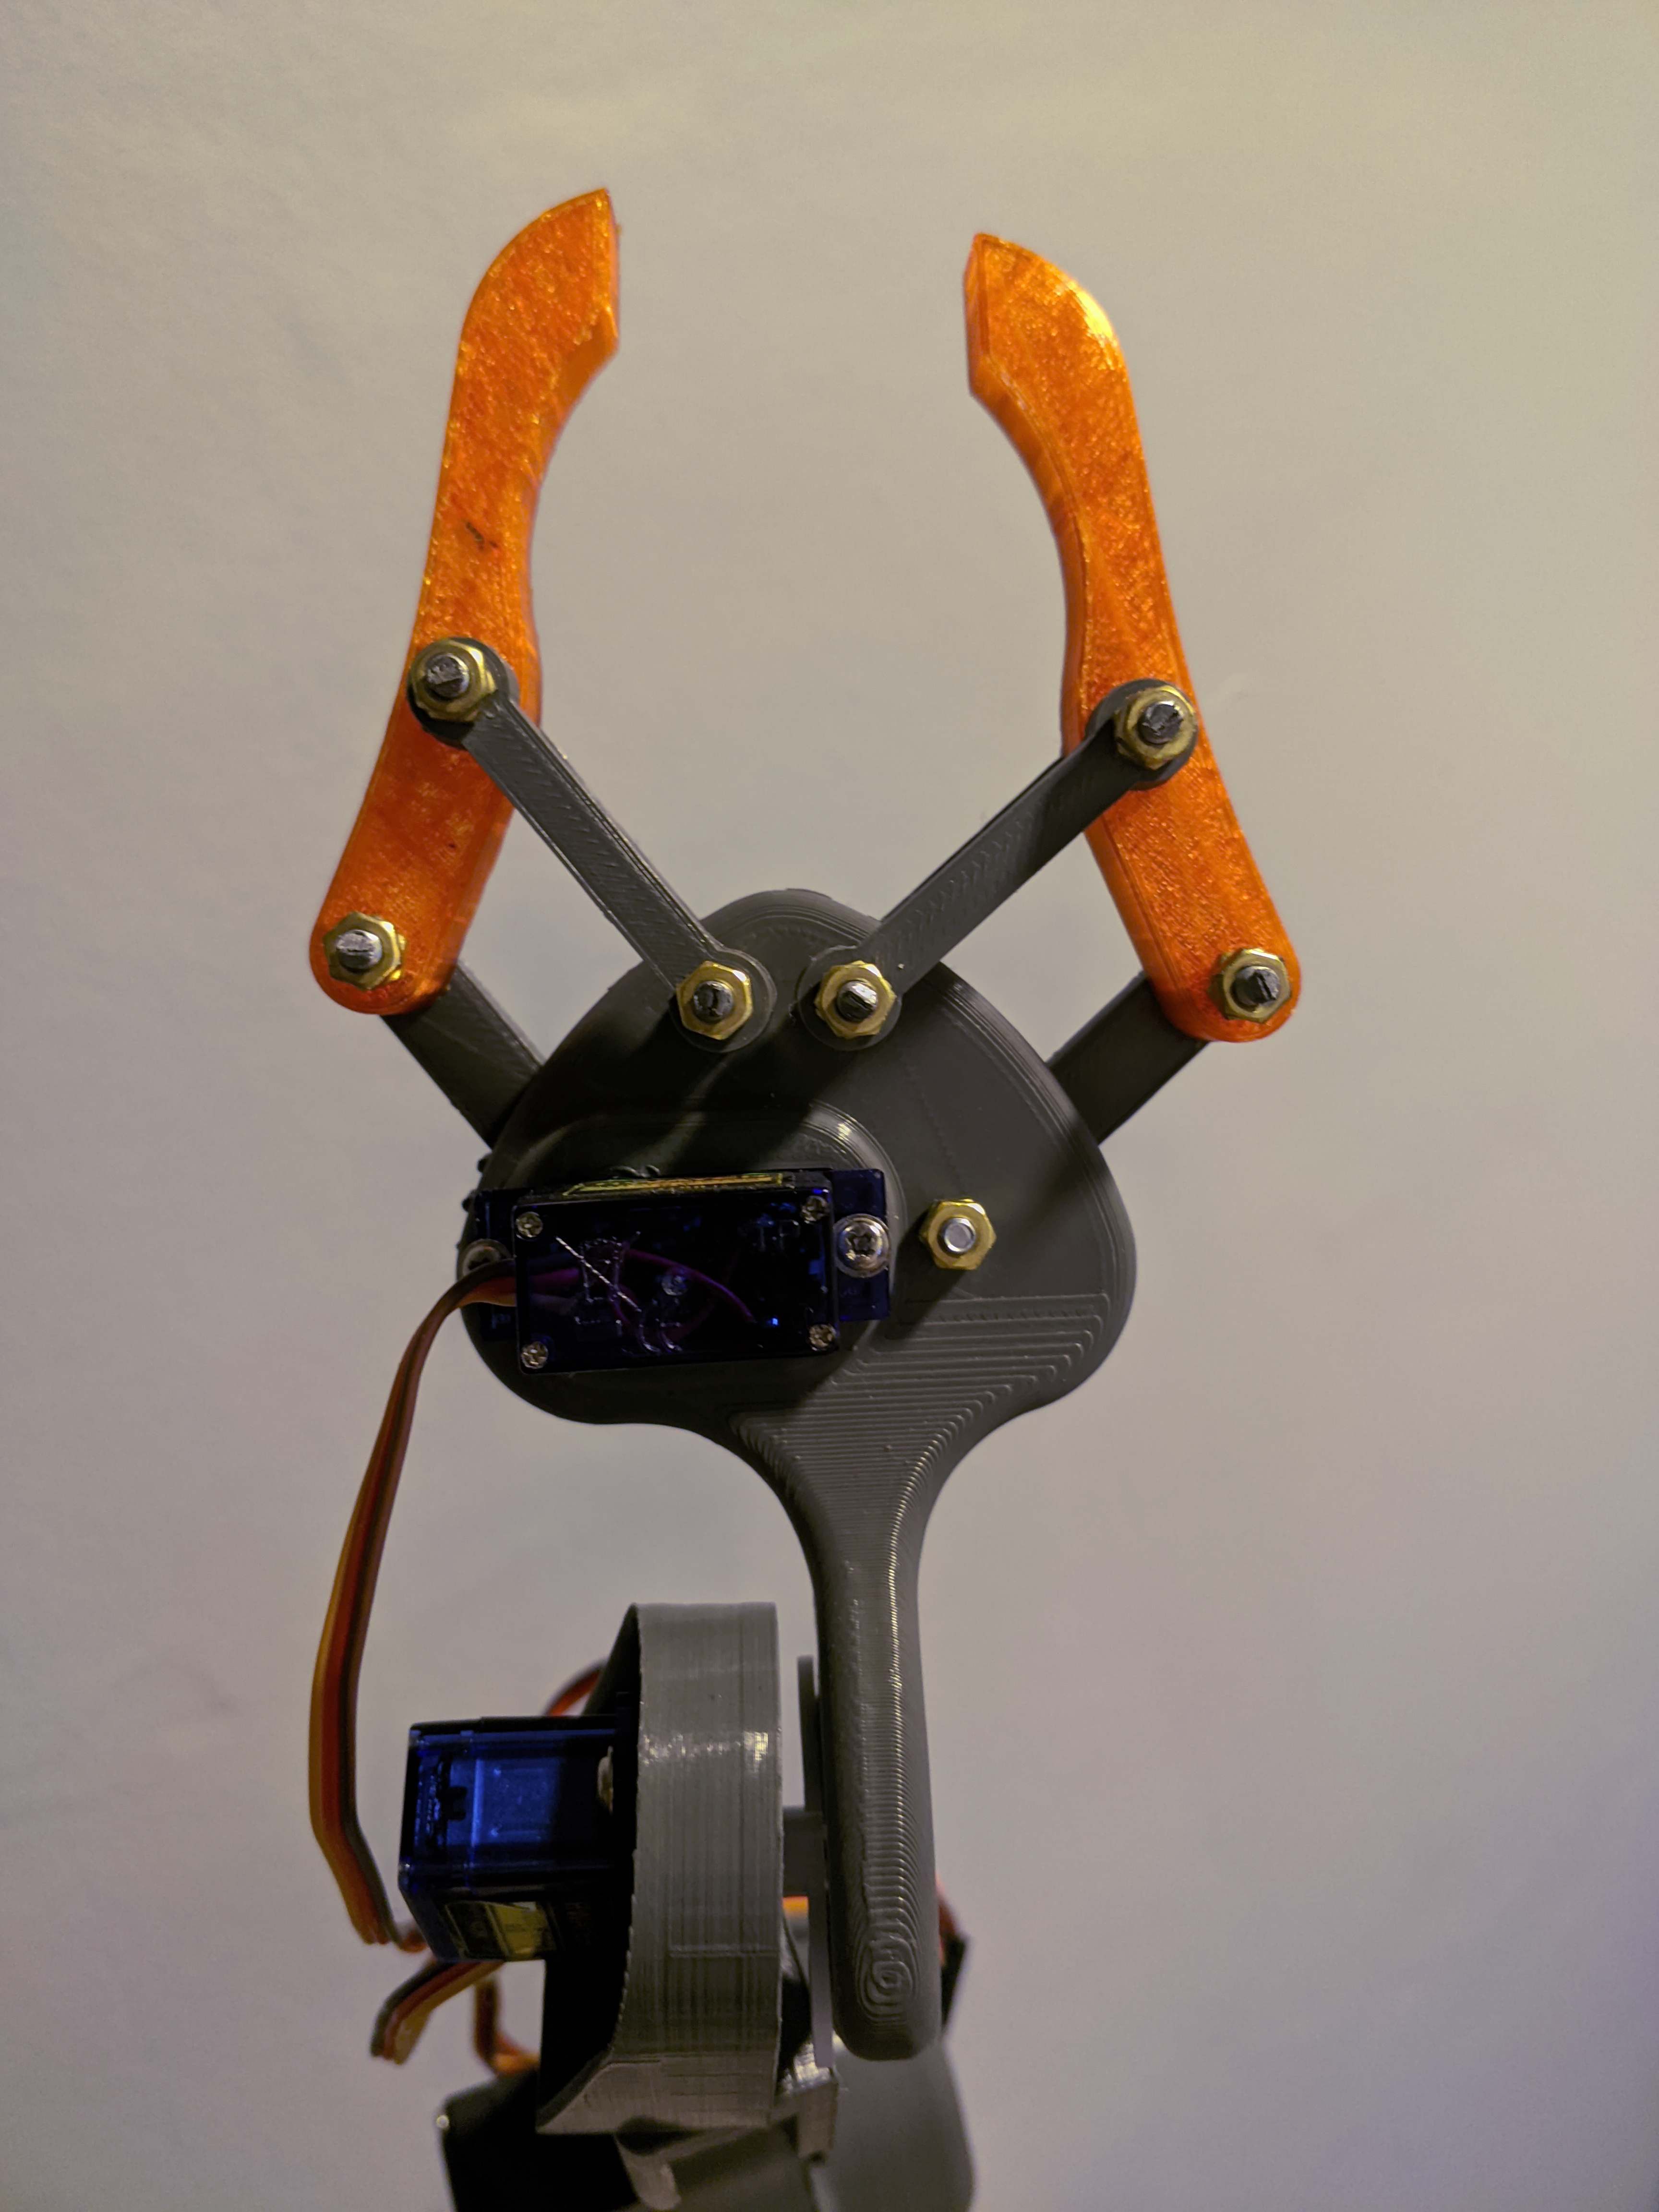
\includegraphics[width=0.8\textwidth]{img/mechC.jpg}
    \end{center}
    \caption{Konstrukcja mechaniczna — chwytak}
    \label{mechC}
\end{figure}

\begin{figure}[p]
    \begin{center}
        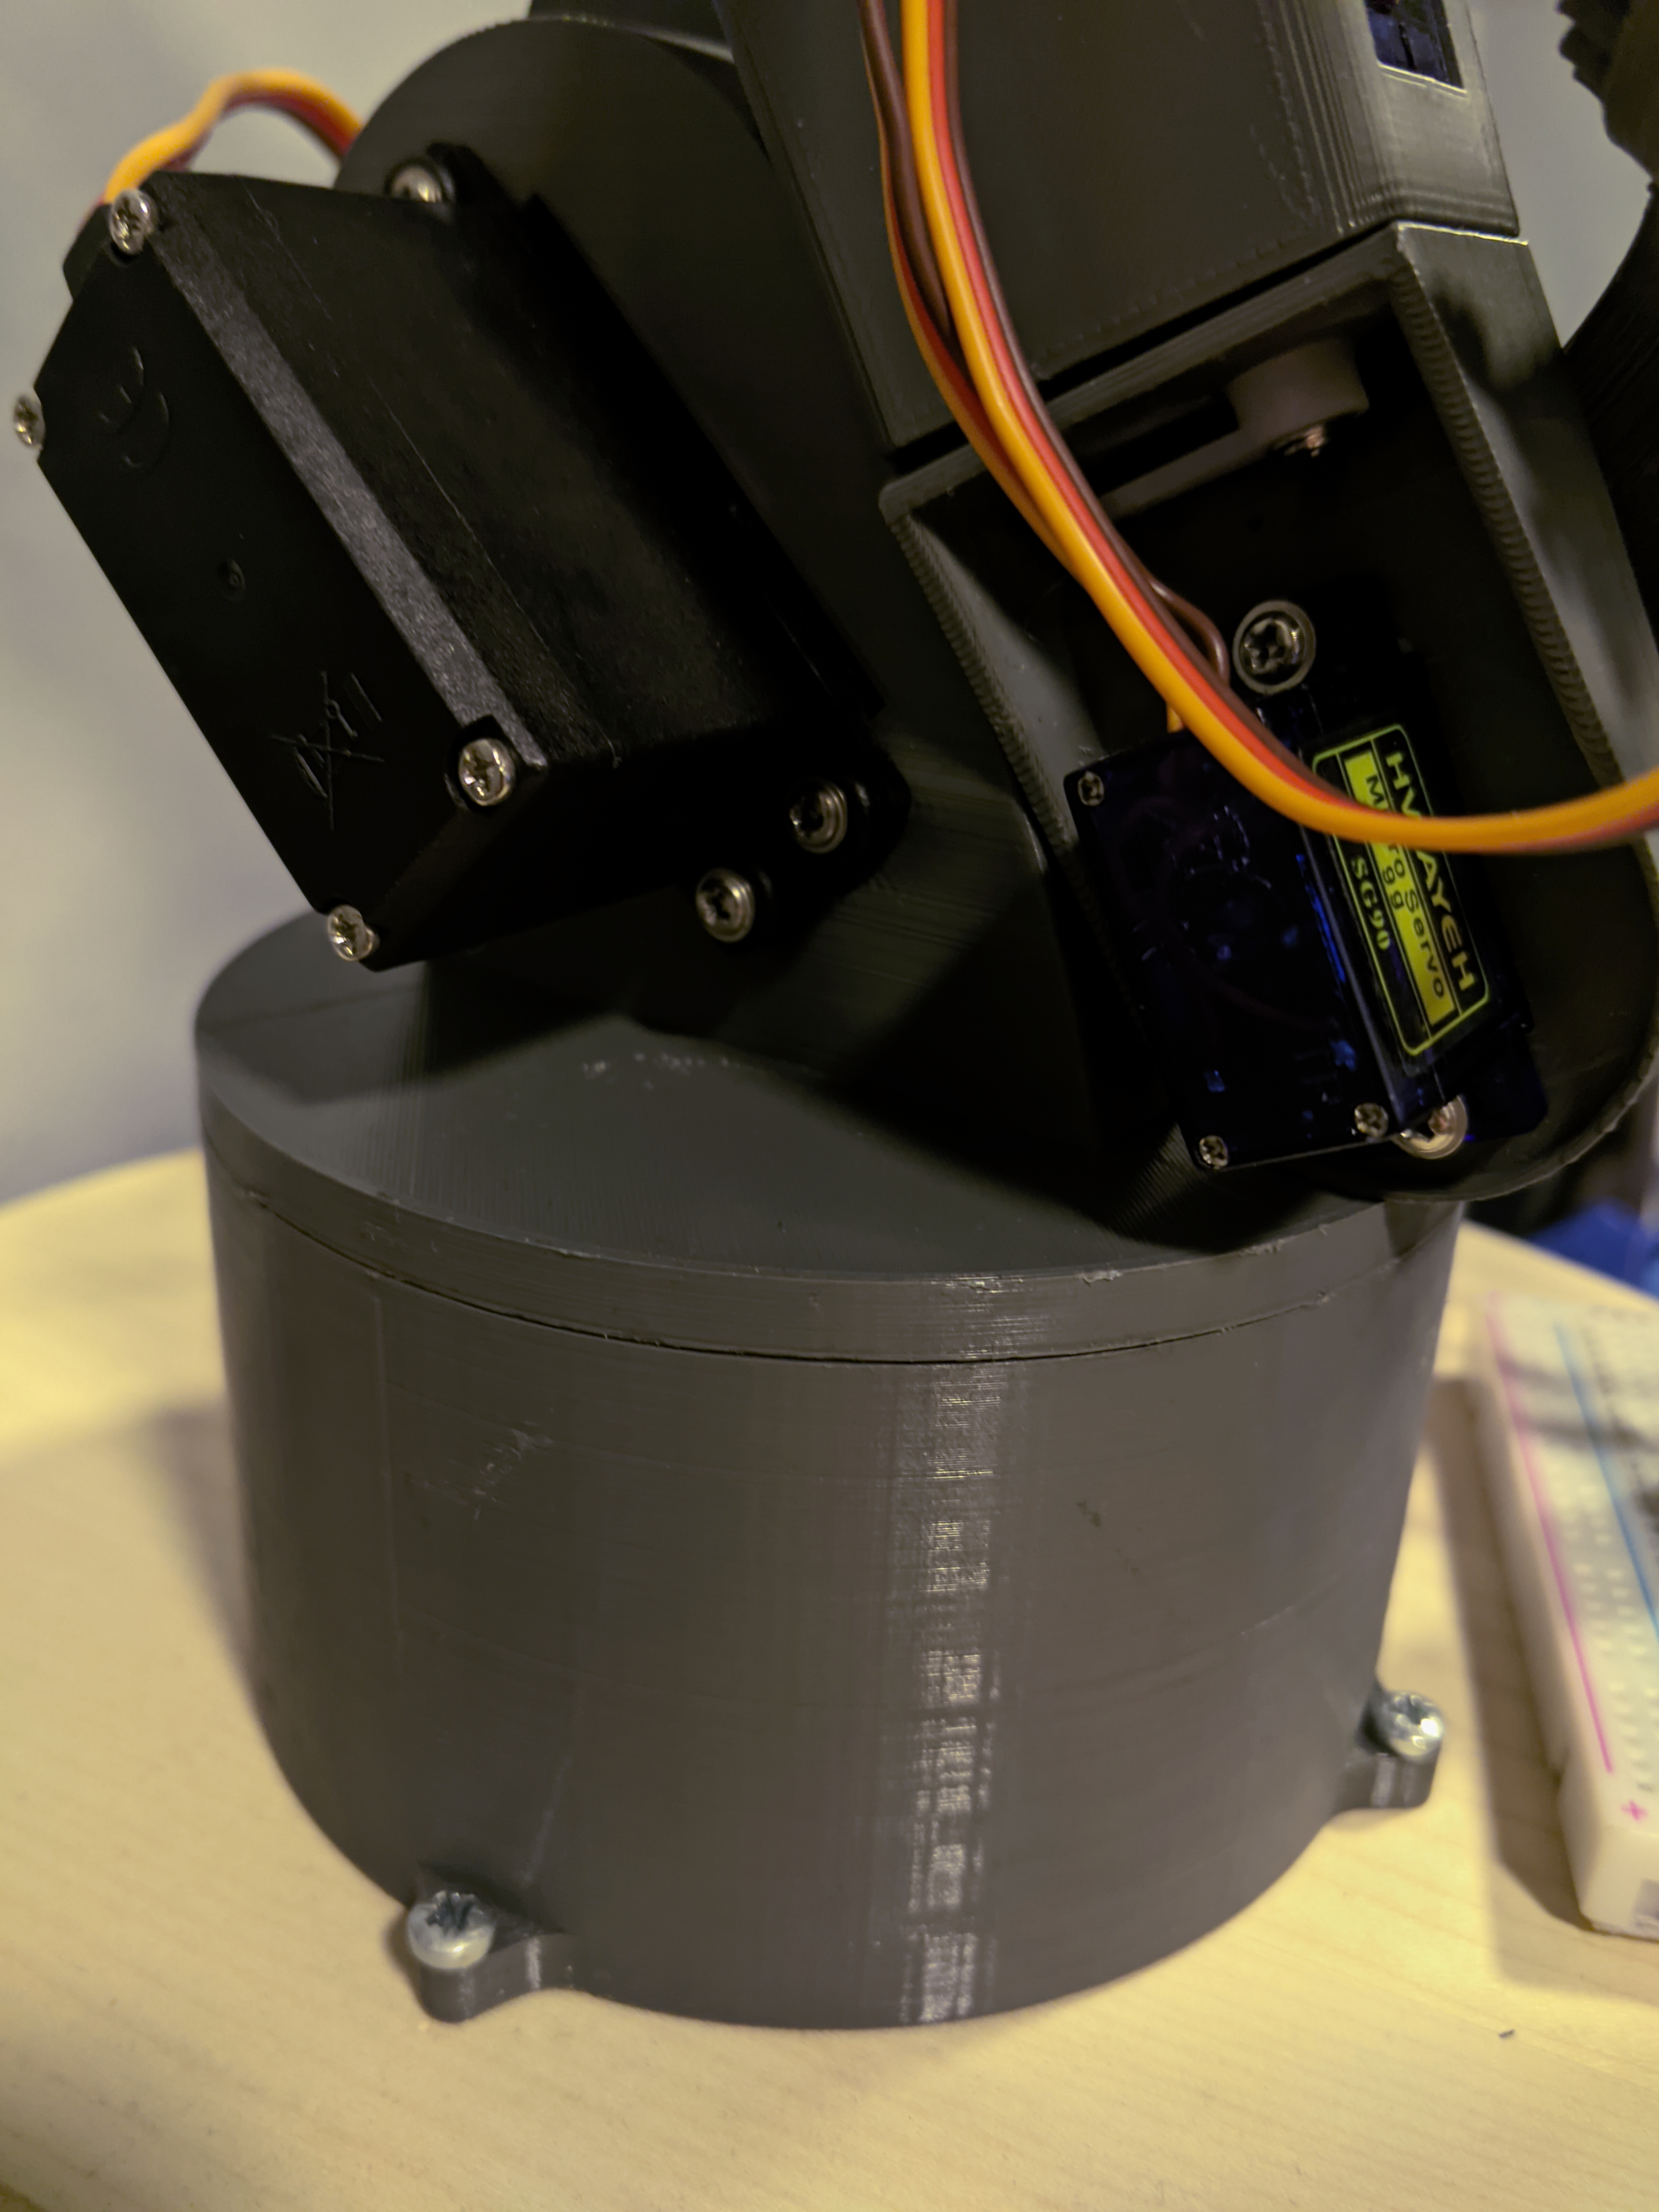
\includegraphics[width=0.9\textwidth]{img/mechB.jpg}
    \end{center}
    \caption{Konstrukcja mechaniczna — podstawa}
    \label{mechB}
\end{figure}

\newpage

\subsubsection{Aplikacja}

Aplikacja powstała w \href{https://appinventor.mit.edu}{\underline{MIT App Inventor}}\footnote{Zintegrowane środowisko programistyczne do tworzenia aplikacji mobilnych} (Rysunki \ref{MITapp} i \ref{MITblocks}). Środowisko to oferuje prostotę w realizacji projektów. Nie wymaga żadnego doświadczenia od użytkownika. Programowanie odbywa się we własnym języku graficznym (duże podobieństwo do \href{https://scratch.mit.edu}{\underline{Scratch}}\footnote{Interpretowany wizualny język programowania}). Kod dostarczonej aplikacji pokazano na Załącznikach \ref{AppBluetooth}, \ref{AppPrzyciski}, \ref{AppSlidery} i \ref{AppKomendy}. Na Rysunku \ref{FinalApp} przedstawiono ostateczną szatę graficzną aplikacji, a na Rysunku \ref{logoapp} zademonstrowano logo aplikacji.

\begin{figure}[h!]
    \begin{center}
        \includegraphics[width=0.7\textwidth]{img/app_src/MITapp.png}
    \end{center}
    \caption{MIT App Inventor — aplikacja}
    \label{MITapp}
\end{figure}

\begin{figure}[h!]
    \begin{center}
        \includegraphics[width=0.7\textwidth]{img/app_src/MITblocks.png}
    \end{center}
    \caption{MIT App Inventor — kod}
    \label{MITblocks}
\end{figure}

\begin{figure}[p]
    \begin{center}
        \includegraphics[width=0.6\textwidth]{img/app.png}
    \end{center}
    \caption{Gotowa aplikacja}
    \label{FinalApp}
\end{figure}

\begin{figure}[p]
    \begin{center}
        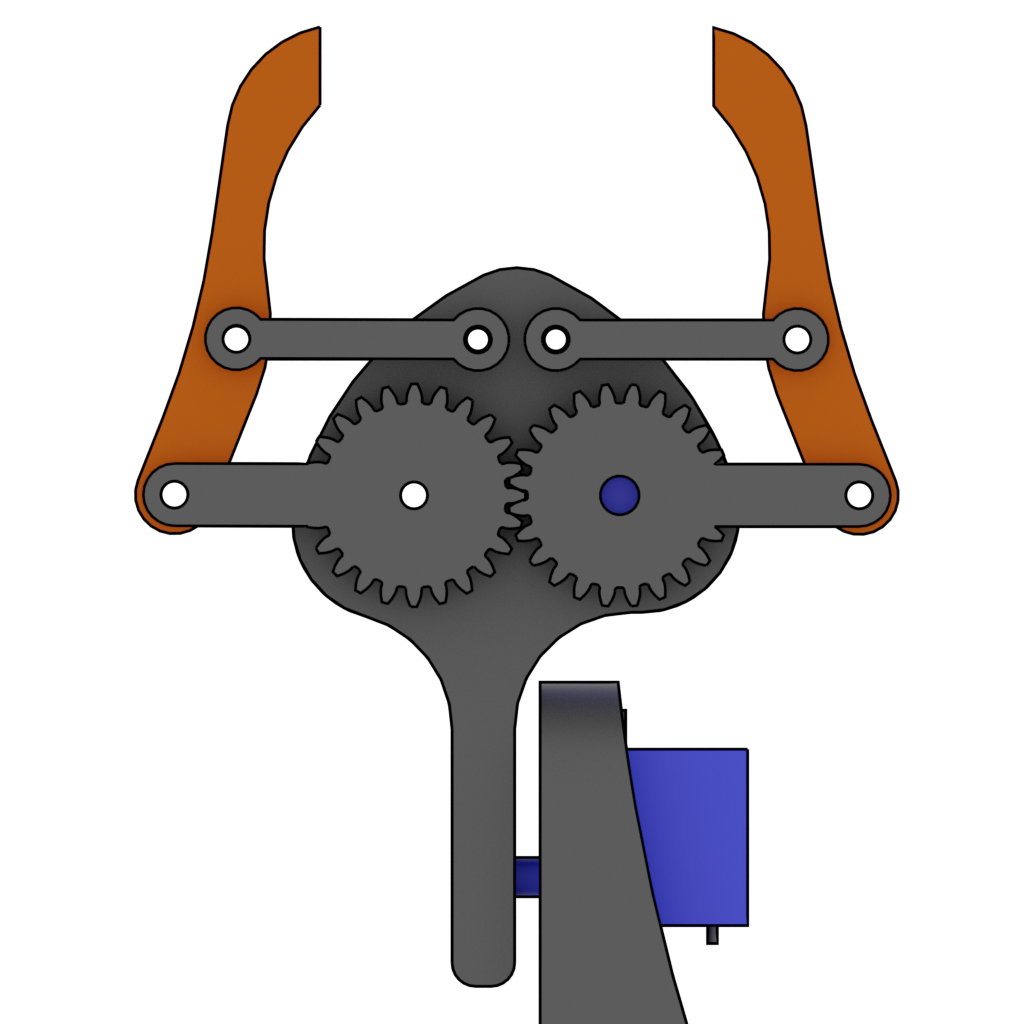
\includegraphics[width=0.8\textwidth]{img/ico.png}
    \end{center}
    \caption{Logo aplikacji}
    \label{logoapp}
\end{figure}

\subsubsection{Protokół komunikacyjny}

Komunikacja aplikacji mobilnej z mikrokontrolerem odbywa się poprzez protokół Bluetooth. Każdy komunikat to odpowiednio sformatowany string. Komendy komunikacyjne przedstawiono w Tabeli \ref{Komunikacja}. Przykładowe komunikaty:
\begin{itemize}
    \item \enquote{s1128n} - ustawienie serwomechanizmu 1 na pozycję 128
    \item \enquote{s564n} - ustawienie serwomechanizmu 5 na pozycję 64
    \item \enquote{c1n} - zapisanie aktualnej pozycji serwomechanizmów w pamięci do późniejszego odtworzenia
    \item \enquote{c4n} - wyczyszczenie zapisanej sekwencji ruchowej
\end{itemize}

\vspace{\fill}

\begin{table}[h!]
    \begin{center}
        \begin{tabular}{|c|c|c|m{10cm}|}
            \hline
            Komenda & Numer & Wartość & Funkcja                                                                                   \\
            \hline
            s       & 1     & x       & Ustawienie serwomechanizmu na pozycję x                                                   \\
            \hline
            s       & 2     & x       & Ustawienie serwomechanizmu na pozycję x                                                   \\
            \hline
            s       & 3     & x       & Ustawienie serwomechanizmu na pozycję x                                                   \\
            \hline
            s       & 4     & x       & Ustawienie serwomechanizmu na pozycję x                                                   \\
            \hline
            s       & 5     & x       & Ustawienie serwomechanizmu na pozycję x                                                   \\
            \hline
            s       & 6     & x       & Ustawienie serwomechanizmu na pozycję x                                                   \\
            \hline
            c       & 1     & -       & Save — zapisanie aktualnej pozycji serwomechanizmów w pamięci do późniejszego odtworzenia \\
            \hline
            c       & 2     & -       & Play — odtwarzanie zapisanej sekwencji ruchowej                                           \\
            \hline
            c       & 3     & -       & Stop — koniec odtwarzania zapisanej sekwencji ruchowej                                    \\
            \hline
            c       & 4     & -       & Reset — wyczyszczenie zapisanej sekwencji ruchowej                                        \\
            \hline
        \end{tabular}
    \end{center}
    \caption{Protokół komunikacyjny}
    \label{Komunikacja}
\end{table}

\vspace{\fill}

\newpage

\section{Podsumowanie}

\subsection{Zrealizowane założenia}

Wszystkie założenia projektowe zostały zrealizowane. Model stworzonego manipulatora przedstawiono na Rysunku \ref{manipulator}.

\begin{figure}[h!]
    \begin{center}
        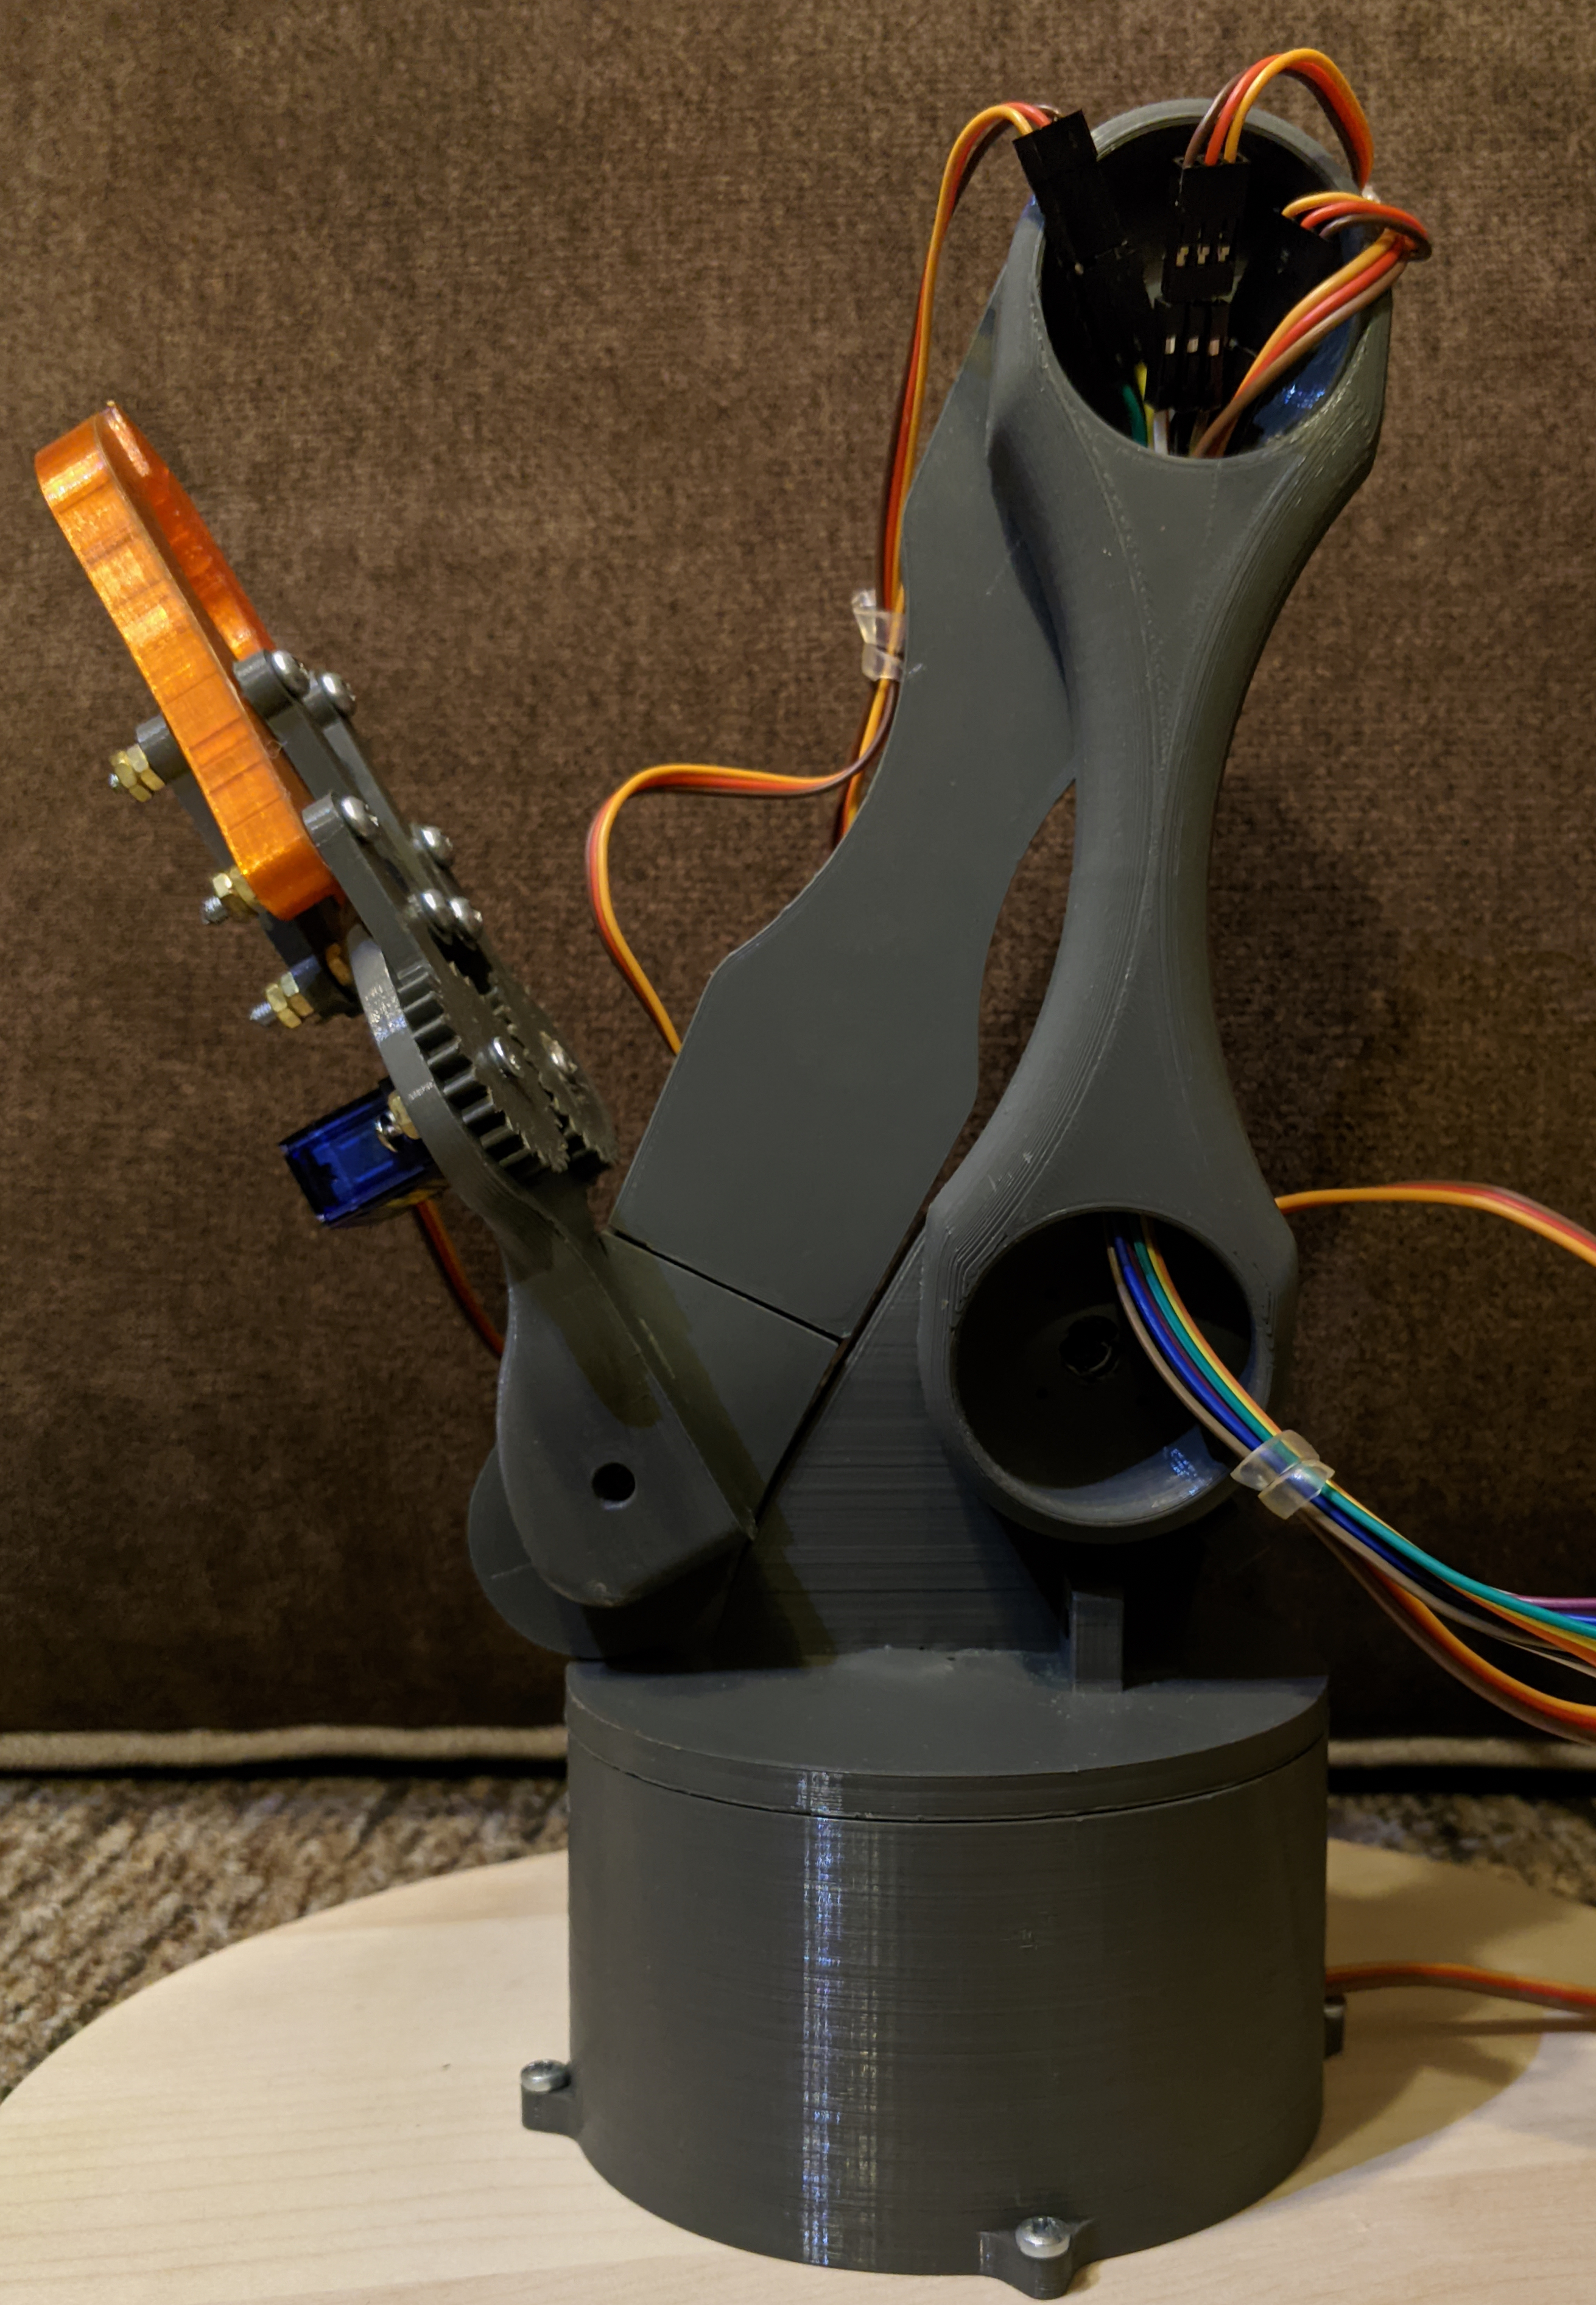
\includegraphics[width=0.374\textwidth]{img/folded.jpg}
        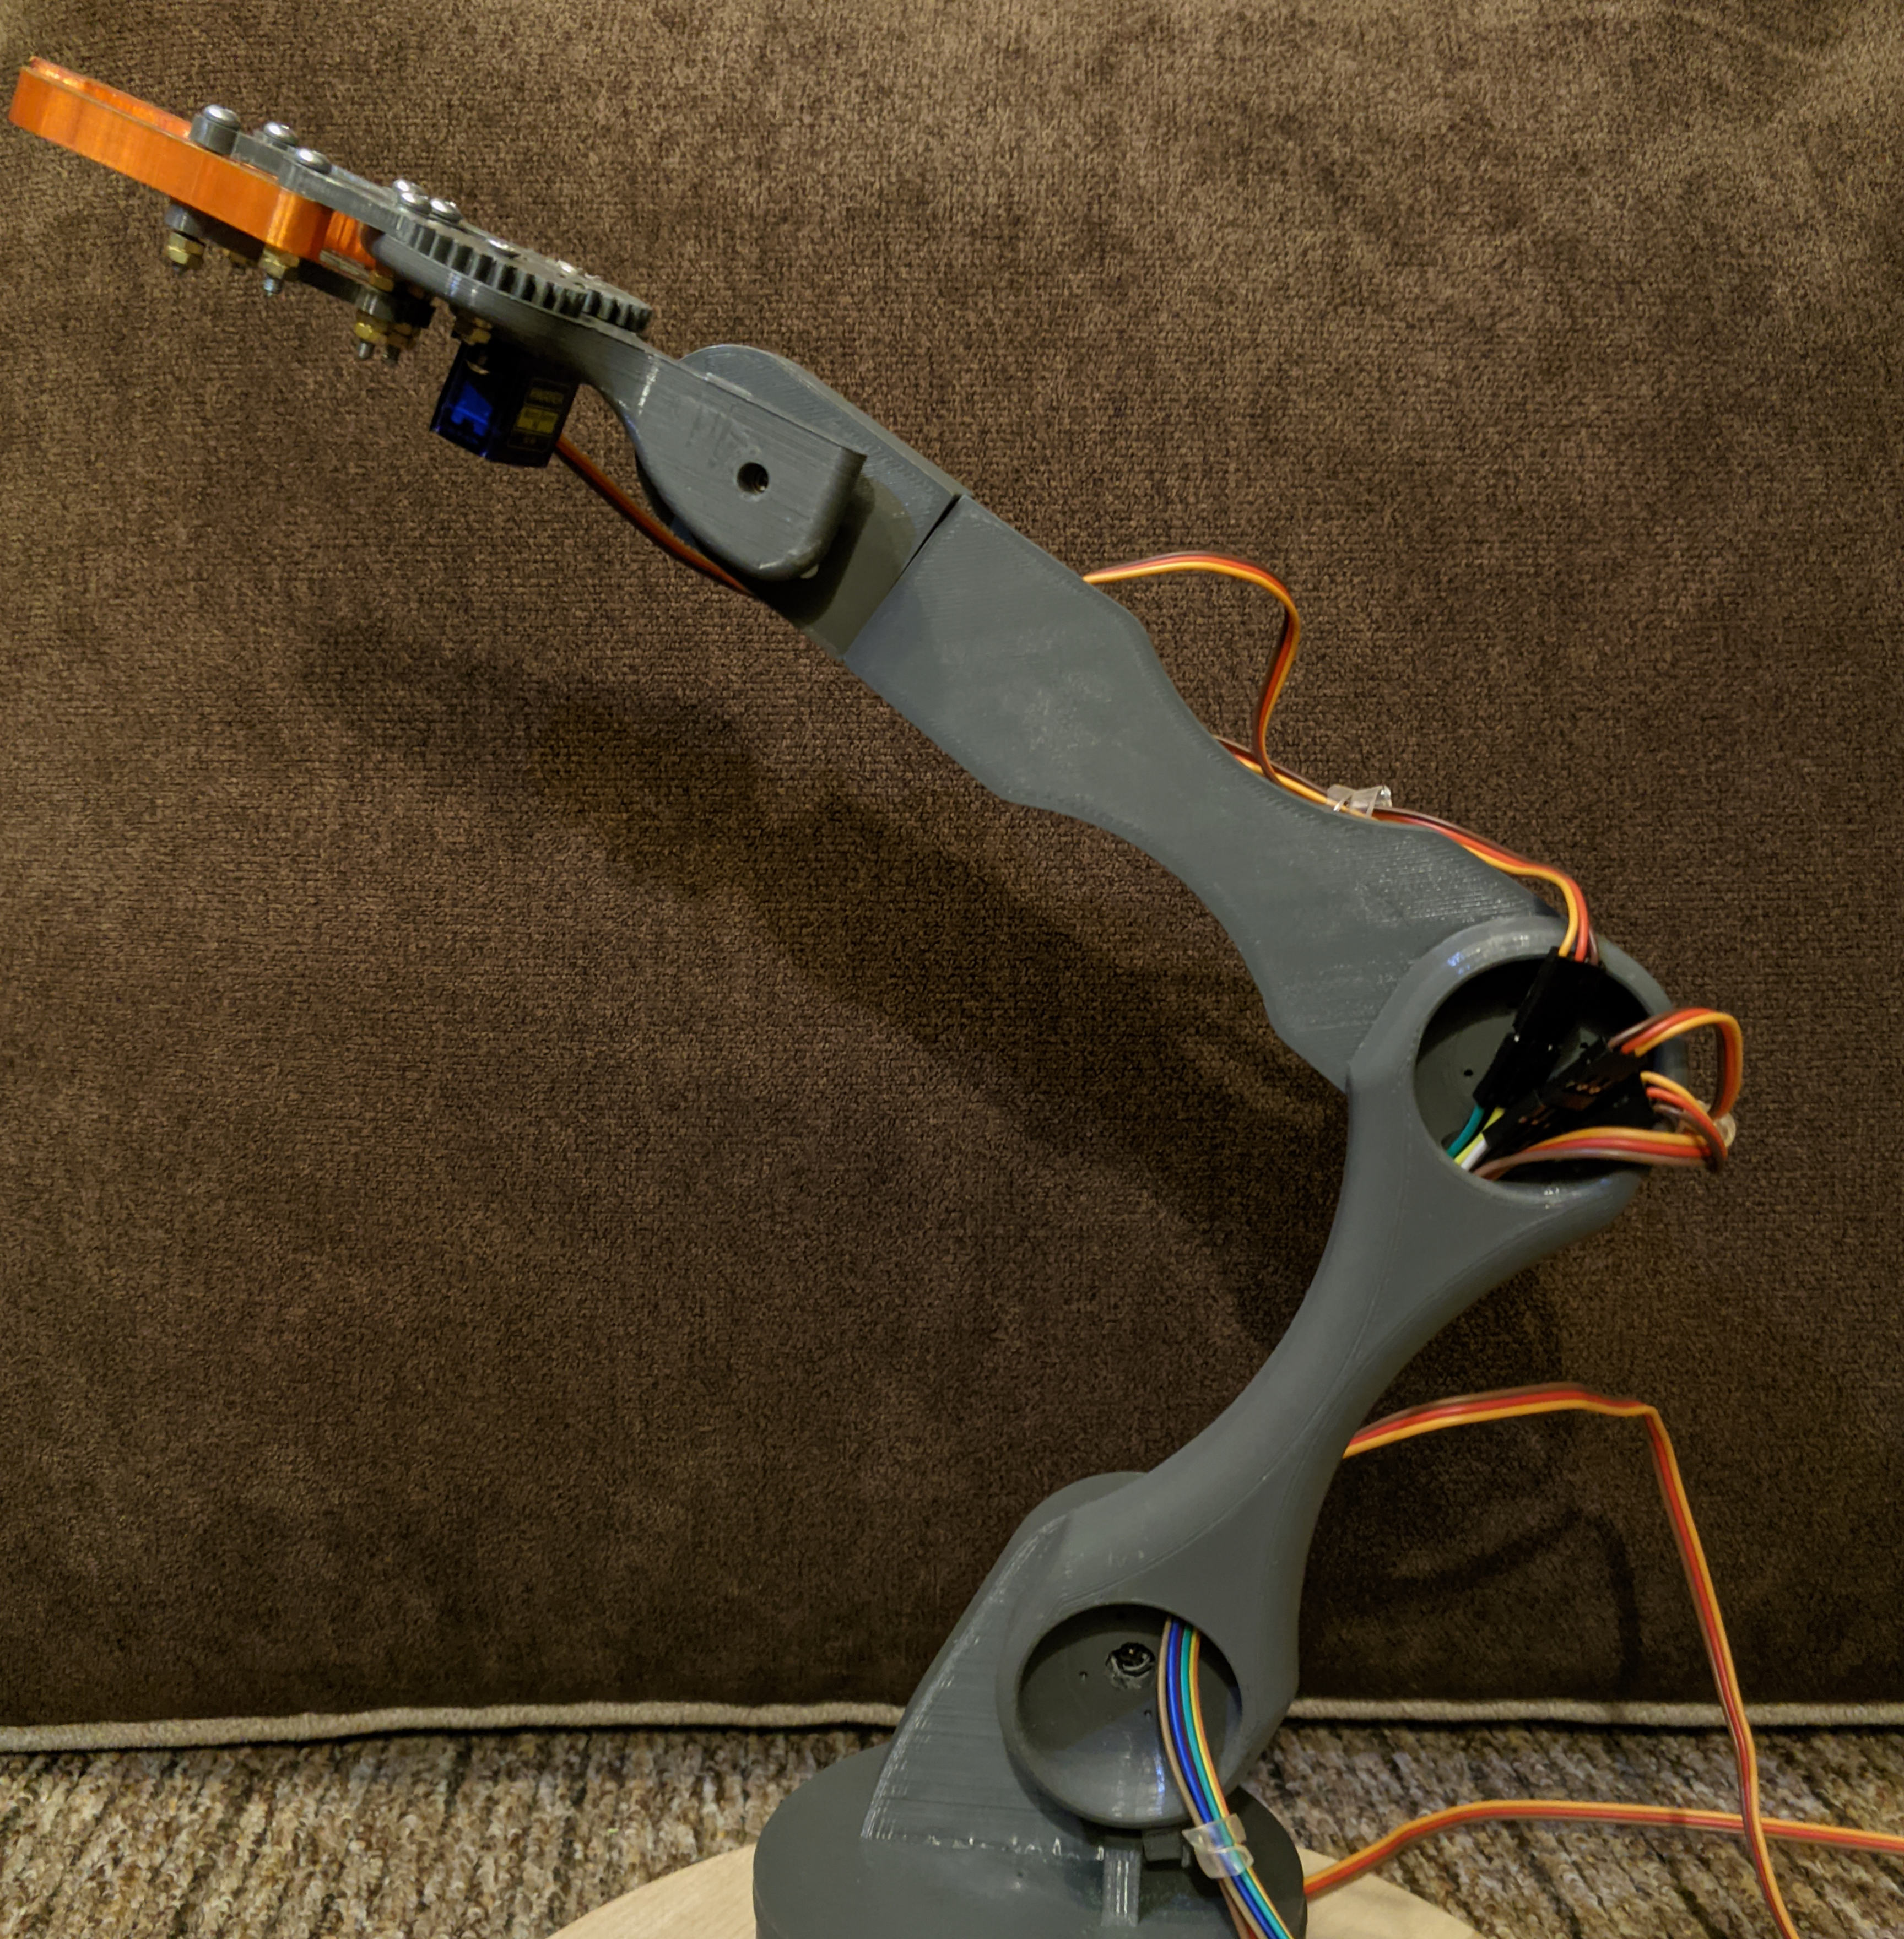
\includegraphics[width=0.53\textwidth]{img/unfolded.jpg}
    \end{center}
    \caption{Model stworzonego manipulatora}
    \label{manipulator}
\end{figure}

\subsection{Poprawki}

Najważniejszą poprawką, którą można zastosować, jest zmiana modelu 3D. W kolejnej wersji należy uwzględnić tolerancje mechaniczne druku oraz nabyte doświadczenie.

\subsection{Dalszy rozwój}

Propozycje dalszego rozwoju:
\begin{itemize}
    \item Zastosowanie wyżej wymienionych poprawek.
    \item Implementacja enkoderów cyfrowych na każdej z osi w celu uzyskania sprzężenia zwrotnego.
    \item Rozwój funkcjonalności aplikacji mobilnej.
    \item Aplikacja mobilna na inne systemy operacyjne.
    \item Zastosowanie kinematyki odwrotnej.
    \item Alternatywne formy sterowania.
\end{itemize}

\newpage

\section{Załączniki}

\renewcommand*{\lstlistingname}{Załącznik}
\renewcommand*{\figurename}{Załącznik}
\setcounter{figure}{2}

\lstinputlisting[style=MyC++Style,label={KodMikrokontrolera},caption={Kod mikrokontrolera}]{../src/main.cpp}

\newpage

\begin{figure}[p]
    \begin{center}
        \includegraphics[width=0.7\textwidth]{img/app_src/bluetooth/BluetoothListBefore.png}
        \includegraphics[width=0.7\textwidth]{img/app_src/bluetooth/BluetoothListAfter.png}
        \includegraphics[width=0.7\textwidth]{img/app_src/bluetooth/BluetoothDisconnected.png}
        \includegraphics[width=0.7\textwidth]{img/app_src/bluetooth/BluetoothClient.png}
    \end{center}
    \caption{Kod aplikacji — Bluetooth}
    \label{AppBluetooth}
\end{figure}

\newpage

\begin{figure}[p]
    \begin{center}
        \includegraphics[width=0.9\textwidth]{img/app_src/posButtons/bttnRotation.png}
        \includegraphics[width=0.9\textwidth]{img/app_src/posButtons/bttnWaist.png}
        \includegraphics[width=0.9\textwidth]{img/app_src/posButtons/bttnElbow.png}
        \includegraphics[width=0.9\textwidth]{img/app_src/posButtons/bttnWristRoll.png}
        \includegraphics[width=0.9\textwidth]{img/app_src/posButtons/bttnWristPitch.png}
        \includegraphics[width=0.9\textwidth]{img/app_src/posButtons/bttnGrip.png}
    \end{center}
    \caption{Kod aplikacji — Przyciski}
    \label{AppPrzyciski}
\end{figure}

\newpage

\begin{figure}[p]
    \begin{center}
        \includegraphics[width=0.8\textwidth]{img/app_src/sliders/slidRotation.png}
        \includegraphics[width=0.8\textwidth]{img/app_src/sliders/slidWaist.png}
        \includegraphics[width=0.8\textwidth]{img/app_src/sliders/slidElbow.png}
        \includegraphics[width=0.8\textwidth]{img/app_src/sliders/slidWristRoll.png}
        \includegraphics[width=0.8\textwidth]{img/app_src/sliders/slidWristPitch.png}
        \includegraphics[width=0.8\textwidth]{img/app_src/sliders/slidGrip.png}
    \end{center}
    \caption{Kod aplikacji — Slidery}
    \label{AppSlidery}
\end{figure}

\newpage

\begin{figure}[p]
    \begin{center}
        \includegraphics[width=0.65\textwidth]{img/app_src/commands/Save.png}
        \includegraphics[width=0.65\textwidth]{img/app_src/commands/Play.png}
        \includegraphics[width=0.65\textwidth]{img/app_src/commands/Stop.png}
        \includegraphics[width=0.65\textwidth]{img/app_src/commands/Reset.png}
    \end{center}
    \caption{Kod aplikacji — Komendy}
    \label{AppKomendy}
\end{figure}

\end{document}